\documentclass[final]{beamer}
%% Possible paper sizes: a0, a0b, a1, a2, a3, a4.
%% Possible orientations: portrait, landscape
%% Font sizes can be changed using the scale option.
\usepackage[size=a0,orientation=portrait,scale=1.3]{beamerposter}

\usetheme{gemini}
% \usecolortheme{seagull}
% \usecolortheme{heriotwatt}
\usecolortheme{um}
% \usecolortheme{cam}
% \usecolortheme{gemini}
% \usecolortheme{labsix}
% \usecolortheme{mit}
\useinnertheme{rectangles}

% ====================
% Packages
% ====================

\usepackage[utf8]{inputenc}
\usepackage{graphicx}
\usepackage{booktabs}
\usepackage{tikz}
\usepackage{pgfplots}
\usepackage{chemformula,array}
\usepackage[version=4]{mhchem}
\usepackage{physics}
\usepackage{braket}

% ====================
% New commands
% ====================
\newcommand{\sepvert}{0.5cm}

% ====================
% Lengths
% ====================

% If you have N columns, choose \sepwidth and \colwidth such that
% (N+1)*\sepwidth + N*\colwidth = \paperwidth
\newlength{\sepwidth}
\newlength{\colwidth}
\setlength{\sepwidth}{0.03\paperwidth}
\setlength{\colwidth}{0.45\paperwidth}

\newcommand{\separatorcolumn}{\begin{column}{\sepwidth}\end{column}}

% ====================
% Logo (optional)
% ====================

% LaTeX logo taken from https://commons.wikimedia.org/wiki/File:LaTeX_logo.svg
% use this to include logos on the left and/or right side of the header:
\logoright{\includegraphics[height=5cm]{logos/UM.pdf}}
\logoleft{
\includegraphics[height=5cm]{logos/TCCM.pdf}}

% ====================
% Footer (optional)
% ====================

\footercontent{
	Europlanet Summer School 2023
	% ``Space missions: ground-based observations and science communication''
	,
	Molėtai Astronomical Observatory (ITPA VU),
	Lithuania
	\hfill
	August 8 - 18, 2023
	\hfill
	\href{mailto:joseantonio.quinonerog@um.es}{\texttt{joseantonio.quinonerog@um.es}}
}
% (can be left out to remove footer)

% ====================
% My own customization
% - BibLaTeX
% - Boxes with tcolorbox
% - User-defined commands
% ====================
\input{custom-defs.tex}

%% Reference Sources
\addbibresource{refs.bib}
\renewcommand{\pgfuseimage}[1]{\includegraphics[scale=2.0]{#1}}

\title{Exploring Quantum Tunnelling in \ch{NH3}}

\author{José A. Quiñonero
	% (\href{mailto:joseantonio.quinonerog@um.es}{\texttt{joseantonio.quinonerog@um.es}})
	\and José Zúñiga
}
	

\institute[shortinst]{Departamento de Química Física, Universidad de Murcia}

\date{August 8 - 18, 2023}

\begin{document}
	
\begin{frame}[t]
	
	\begin{columns}[t]

		\begin{column}{2\colwidth+\sepwidth}

		\textit{Tunnelling is present since the evolution of the primitive Universe,
		allowing the origin and evolution of life.}

		\end{column}

	\end{columns}

	\begin{columns}[t]
		\separatorcolumn
		
		\begin{column}{\colwidth}

			\begin{block}{Introduction and main objective}
				\begin{itemize}
					\item \textbf{Visualize tunnelling, in real time, with your own eyes}

						\vspace{\sepvert}
						\begin{figure}[tb!]
							\centering
							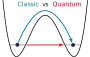
\includegraphics[width=0.4\textwidth]{figures/classic-vs-quantum.pdf}
							% \subimport{figures/}{.pgf}
						\end{figure}
						\vspace{\sepvert}

					\item Study tunnelling in a realistic example, the inversion motion of
						\ch{NH3}, which gave birth to the first MASER

						\vspace{\sepvert}
						\begin{figure}[tb!]
							\centering
							\includegraphics[width=0.9\textwidth]{figures/esquema_inversion.pdf}
							% \subimport{figures/}{.pgf}
						\end{figure}
						\vspace{\sepvert}

					\item \textbf{Double symmetric potential well:} lower energy
						equilibrium $C_{3v}$ (wells) and higher energy $D_{3h}$ 
						(barrier)

				\end{itemize}
			\end{block}
			
			\begin{alertblock}{Hammiltonian}
				\vspace{-\sepvert} \hrule \vspace{0.8cm}
			
				\begin{equation*}
					\hat{H} =
					- \frac{ \hbar^2 }{2 \mu} \frac{ \dd^2 }{ \dd{x^2} } +
					\frac{V_b}{x_e^4} x^4 - \frac{2V_b}{x_e^2} x^2 + V_b
				\end{equation*}

			\end{alertblock}
			
			\begin{exampleblock}{Hola}
				VidaVidaVidaVidaVidaVidaVidaVidaVidaVidaVidaVidaVidaVida
			\end{exampleblock}

			\begin{xmybox}{Hola}
				VidaVidaVidaVidaVidaVidaVidaVidaVidaVidaVidaVidaVidaVida
			\end{xmybox}
			
			\begin{defbox}{Hola}
				VidaVidaVidaVidaVidaVidaVidaVidaVidaVidaVidaVidaVidaVida
			\end{defbox}

			\begin{infobox}{Hola}
				VidaVidaVidaVidaVidaVidaVidaVidaVidaVidaVidaVidaVidaVida
			\end{infobox}

			\begin{exabox}{Hola}
				VidaVidaVidaVidaVidaVidaVidaVidaVidaVidaVidaVidaVidaVida
			\end{exabox}

			\begin{thm}{title}{nameref}
				contents
			\end{thm}

			\begin{prop}{title}{nameref}
				contents
			\end{prop}

			\begin{conj}{title}{nameref}
				contents
			\end{conj}

			\begin{lem}{title}{nameref}
				contents
			\end{lem}

			\begin{clm}{title}{nameref}
				contents
			\end{clm}

			\begin{block}{Fusce aliquam magna velit}
				
				Et rutrum ex euismod vel. Pellentesque ultricies, velit in fermentum
				vestibulum, lectus nisi pretium nibh, sit amet aliquam lectus augue vel
				velit. 
				
				\begin{enumerate}
					\item \textbf{Morbi mauris purus}, egestas at vehicula et, convallis
					accumsan orci. Orci varius natoque penatibus et magnis dis parturient
					montes, nascetur ridiculus mus.
					\item \textbf{Cras vehicula blandit urna ut maximus}. Aliquam blandit nec
					massa ac sollicitudin. Curabitur cursus, metus nec imperdiet bibendum,
					velit lectus faucibus dolor, quis gravida metus mauris gravida turpis.
				\end{enumerate}
				
				\begin{figure}
					\centering
					\begin{tikzpicture}
						\begin{axis}[
							scale only axis,
							no markers,
							domain=0:2*pi,
							samples=100,
							axis lines=center,
							axis line style={-},
							ticks=none]
							\addplot[red] {sin(deg(x))};
							\addplot[blue] {cos(deg(x))};
						\end{axis}
					\end{tikzpicture}
					\caption{Another figure caption.}
				\end{figure}
				
			\end{block}
			
		\end{column}
	
		\separatorcolumn
		
		\begin{column}{\colwidth}
			
			\begin{block}{Nam cursus consequat egestas}
				
				\begin{itemize}
					\item \textbf{Sed consequat} id ante vel efficitur. Praesent congue massa
					sed est scelerisque, elementum mollis augue iaculis.
					\begin{itemize}
						\item In sed est finibus, vulputate
						nunc gravida, pulvinar lorem. In maximus nunc dolor, sed auctor eros
						porttitor quis.
						\item Fusce ornare dignissim nisi. Nam sit amet risus vel lacus
						tempor tincidunt eu a arcu.
						\item Donec rhoncus vestibulum erat, quis aliquam leo
						gravida egestas.
					\end{itemize}
					\item \textbf{Sed luctus, elit sit amet} dictum maximus, diam dolor
					faucibus purus, sed lobortis justo erat id turpis.
					\item \textbf{Pellentesque facilisis dolor in leo} bibendum congue.
					Maecenas congue finibus justo, vitae eleifend urna facilisis at.
				\end{itemize}
				
			\end{block}
			
			\begin{exampleblock}{An example block containing some math}{}
				
				Nullam non est elit. In eu ornare justo. Maecenas porttitor sodales lacus,
				ut cursus augue sodales ac.
				
				$$
				\int_{-\infty}^{\infty} e^{-x^2}\,dx = \sqrt{\pi}
				$$
				
				\begin{enumerate}
					\item \textbf{Morbi mauris purus}, egestas at vehicula et, convallis
					accumsan orci. Orci varius natoque penatibus et magnis dis parturient
					montes, nascetur ridiculus mus.
					\item \textbf{Cras vehicula blandit urna ut maximus}. Aliquam blandit nec
					massa ac sollicitudin. Curabitur cursus, metus nec imperdiet bibendum,
					velit lectus faucibus dolor, quis gravida metus mauris gravida turpis.
				\end{enumerate}
				
				\heading{A heading inside a block}
				
				Praesent consectetur mi $x^2 + y^2$ metus, nec vestibulum justo viverra
				nec. Proin eget nulla pretium, egestas magna aliquam, mollis neque. Vivamus
				dictum $\mathbf{u}^\intercal\mathbf{v}$ sagittis odio, vel porta erat
				congue sed. Maecenas ut dolor quis arcu auctor porttitor.
				
				\heading{Another heading inside a block}
				
				Sed augue erat, scelerisque a purus ultricies, placerat porttitor neque.
				Donec $P(y \mid x)$ fermentum consectetur $\nabla_x P(y \mid x)$ sapien
				sagittis egestas. Duis eget leo euismod nunc viverra imperdiet nec id
				justo.
				
			\end{exampleblock}
			
			\begin{block}{Nullam vel erat at velit convallis laoreet}
				
				Class aptent taciti sociosqu ad litora torquent per conubia nostra, per
				inceptos himenaeos. Phasellus libero enim, gravida sed erat sit amet,
				scelerisque congue diam. Fusce dapibus dui ut augue pulvinar iaculis.
				
				\begin{table}
					\centering
					\begin{tabular}{l r r c}
						\toprule
						\textbf{First column} & \textbf{Second column} & \textbf{Third column} & \textbf{Fourth} \\
						\midrule
						Foo & 13.37 & 384,394 & $\alpha$ \\
						Bar & 2.17 & 1,392 & $\beta$ \\
						Baz & 3.14 & 83,742 & $\delta$ \\
						Qux & 7.59 & 974 & $\gamma$ \\
						\bottomrule
					\end{tabular}
					\caption{A table caption.}
				\end{table}
				
				Donec quis posuere ligula. Nunc feugiat elit a mi malesuada consequat. Sed
				imperdiet augue ac nibh aliquet tristique. Aenean eu tortor vulputate,
				eleifend lorem in, dictum urna. Proin auctor ante in augue tincidunt
				tempor. Proin pellentesque vulputate odio, ac gravida nulla posuere
				efficitur. Aenean at velit vel dolor blandit molestie. Mauris laoreet
				commodo quam, non luctus nibh ullamcorper in. Class aptent taciti sociosqu
				ad litora torquent per conubia nostra, per inceptos himenaeos.
				
				Nulla varius finibus volutpat. Mauris molestie lorem tincidunt, iaculis
				libero at, gravida ante. Phasellus at felis eu neque suscipit suscipit.
				Integer ullamcorper, dui nec pretium ornare, urna dolor consequat libero,
				in feugiat elit lorem euismod lacus. Pellentesque sit amet dolor mollis,
				auctor urna non, tempus sem.
				
			\end{block}
			
			
			\begin{block}{References}
				\printbibliography[heading=none]
			\end{block}
		\end{column}
		
		\separatorcolumn
	\end{columns}
\end{frame}
\end{document}
